\clearpage
\begin{explanationbox}
\textbf{第一层：用初中几何理解——内角平分线与外角平分线。}

\begin{center}
% P=(0,0) is a translated copy of (2,3); focal rays (-4,-3),(0,-3).
\begin{tikzpicture}[x=.95cm,y=.95cm,>=stealth,font=\small]
\draw[gray,thick] (0,0)--(-4,-3) (0,0)--(0,-3);
\draw[gray,dotted] (0,0)--(0,1.6);
\draw[orange!80!black,thick,dashed] (-1.7,-3.4)--(.9,1.8);
\draw[teal!85!black,thick,dashed] (-3,1.5)--(2,-1);
\draw[orange!80!black] ({.7*cos(216.86989765)},{.7*sin(216.86989765)})
 arc[start angle=216.86989765,end angle=243.43494882,radius=.7];
\draw[orange!80!black] ({.85*cos(243.43494882)},{.85*sin(243.43494882)})
 arc[start angle=243.43494882,end angle=270,radius=.85];
\draw[teal!85!black] (0,1.05) arc[start angle=90,end angle=153.43494882,radius=1.05];
\draw[teal!85!black] ({1.2*cos(153.43494882)},{1.2*sin(153.43494882)})
 arc[start angle=153.43494882,end angle=216.86989765,radius=1.2];
\draw (.268,-.134)--(.402,.134)--(.134,.268);
\fill (0,0) circle (2pt) node[above right=7pt] {$P$};
\fill (-4,-3) circle (2pt) node[below=5pt] {$F_1$};
\fill (0,-3) circle (2pt) node[below right=5pt] {$F_2$};
\node[orange!80!black,above=5pt] at (.9,1.8) {$t_H$：内角平分线};
\node[teal!85!black,anchor=east] at (-2.5,1.7) {$t_E$：外角平分线};
\node at (-1,-4.1) {内、外角平分线夹角为 $90^\circ$};
\end{tikzpicture}


{\small 橙色切线平分内角，青色切线平分外角；两个平分方向垂直。}
\end{center}
图中两条切线互相垂直；椭圆法线沿内角平分线，双曲线法线沿外角平分线。
这里谈的是方向直线，不受所选支别或箭头方向影响。

\textbf{为什么“椭圆对应内、双曲线对应外”？}这并不是另外要死记的结论。
因为椭圆保持两段焦半径\emph{总和}不变，双曲线保持两段焦半径
\emph{之差}不变。下面把它们的变化方向算出来，就能自行推出角平分性质。
\end{explanationbox}

\clearpage
\begin{explanationbox}
\textbf{第二层：把“和、差”真正变成两个方向。}

记 $r_i=PF_i$，从焦点 $F_i$ 指向 $P$ 的\emph{单位向量}为
\[
\mathbf u_i=\frac{\overrightarrow{F_iP}}{PF_i},\qquad
|\mathbf u_1|=|\mathbf u_2|=1.
\]
让 $P$ 沿曲线运动，用 $\mathbf v$ 表示它在 $P$ 处的速度向量，其方向就是切线方向。
把距离关系两边平方后，利用高中导数求得
\[
2r_i r_i'=2\overrightarrow{F_iP}\cdot\mathbf v
\quad\Longrightarrow\quad r_i'=\mathbf u_i\cdot\mathbf v.
\]
这里 $r_i'$ 表示距离的瞬时变化率，且 $r_i>0$。
椭圆上两段距离的和不变；双曲线同一支上两段距离的差不变。
因此相应的切线方向分别满足
\[
(\mathbf u_1+\mathbf u_2)\cdot\mathbf v_E=0,\qquad
(\mathbf u_1-\mathbf u_2)\cdot\mathbf v_H=0.
\]
\textbf{为什么看法线？}法线就是过 $P$ 且垂直于切线的直线。
上面两式说明，两个括号里的向量分别垂直于两条切线，所以
\[
\mathbf n_E\parallel\mathbf u_1+\mathbf u_2,\qquad
\mathbf n_H\parallel\mathbf u_1-\mathbf u_2.
\]
于是
\[
\begin{aligned}
(\mathbf u_1+\mathbf u_2)\cdot(\mathbf u_1-\mathbf u_2)
&=|\mathbf u_1|^2-|\mathbf u_2|^2\\
&=1-1=0.
\end{aligned}
\]
\begin{center}
% u1=(4/5,3/5), u2=(0,1), shown as free vectors based at P.
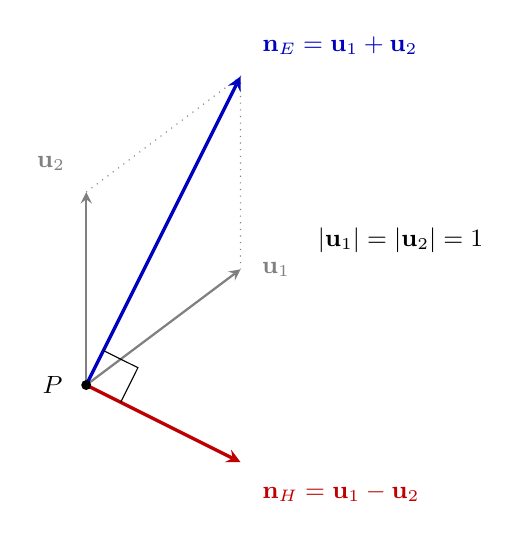
\begin{tikzpicture}[x=2.45cm,y=2.45cm,>=stealth,font=\small]
\draw[gray,dotted] (0,1)--(.8,1.6)--(.8,.6);
\draw[->,gray,thick] (0,0)--(.8,.6) node[right=4pt] {$\mathbf u_1$};
\draw[->,gray,thick] (0,0)--(0,1) node[above left=4pt] {$\mathbf u_2$};
\draw[->,blue!75!black,very thick] (0,0)--(.8,1.6)
 node[above right=4pt] {$\mathbf n_E=\mathbf u_1+\mathbf u_2$};
\draw[->,red!75!black,very thick] (0,0)--(.8,-.4)
 node[below right=4pt] {$\mathbf n_H=\mathbf u_1-\mathbf u_2$};
\draw (.089,.179)--(.268,.09)--(.179,-.089);
\fill (0,0) circle (1.8pt) node[left=5pt] {$P$};
\node[anchor=west] at (1.15,.75) {$|\mathbf u_1|=|\mathbf u_2|=1$};
\end{tikzpicture}


{\small 两单位向量等长，和与差就是两个正交的法线方向。}
\end{center}
\textbf{中学知识迁移：}任意两条等长向量 $\mathbf a,\mathbf b$，
都满足 $(\mathbf a+\mathbf b)\perp(\mathbf a-\mathbf b)$；
这也是菱形两条对角线互相垂直的向量原因。
\end{explanationbox}


\clearpage
\begin{explanationbox}
\textbf{平方关系的来源与用途：为什么“平方差 = 平方和”？}

先写熟悉的两条焦半距公式，不要直接背新等式：
\[
\text{椭圆：}\quad c^2=a^2-b^2,\qquad
\text{双曲线：}\quad c^2=A^2+B^2.
\]
\textbf{为什么令两式相等？}共焦意味着两条曲线的焦点均为
$(-c,0)$、$(c,0)$，所以焦半距 $c$ 是同一个数。
\[
 a^2-b^2=A^2+B^2
 \quad\Longleftrightarrow\quad
 \boxed{a^2-A^2=b^2+B^2}.
\]
\begin{center}
% Two exact right triangles share the SAME segment c.
% Representative lengths: a=5,b=4,c=3,A=9/5,B=12/5.
% O=(0,0), C=(0,3), R=(4,0), Q=(-36/25,27/25).
\begin{tikzpicture}[x=1.15cm,y=1.15cm,font=\normalsize,line join=round]
\coordinate (O) at (0,0);
\coordinate (C) at (0,3);
\coordinate (R) at (4,0);
\coordinate (Q) at (-1.44,1.08);
\fill[blue!5] (O)--(R)--(C)--cycle;
\fill[red!5] (O)--(Q)--(C)--cycle;
\draw[blue!75!black,very thick] (O)--(R) node[midway,below=6pt] {$b$}
    --(C) node[midway,above right=4pt] {$a$};
\draw[red!75!black,very thick] (O)--(Q) node[midway,below left=5pt] {$A$}
    --(C) node[midway,above left=5pt] {$B$};
\draw[black,very thick] (O)--(C) node[midway,right=5pt,align=center] {$c$\\[-1pt]{\small 共用边}};
\draw[blue!75!black,thick] (0,.22)--(.22,.22)--(.22,0);
\draw[red!75!black,thick] (-1.264,.948)--(-1.132,1.124)--(-1.308,1.256);
\node[blue!75!black] at (2.25,3.65) {$a^2=b^2+c^2$};
\node[red!75!black] at (-1.6,3.65) {$c^2=A^2+B^2$};
\end{tikzpicture}


{\small 两个直角三角形共用同一条边 $c$；边长按比例绘制。}
\end{center}
右侧三角形以 $a$ 为斜边、$b,c$ 为直角边；
左侧三角形以共用边 $c$ 为斜边、$A,B$ 为直角边。
把第二次勾股定理代入第一次，即得 $a^2=b^2+A^2+B^2$。
这些是参数构造三角形，$B$ 仍是双曲线虚半轴。

\textbf{逆用边界：}只在已知两条曲线的中心、焦轴和标准坐标系一致时，
$ a^2-A^2=b^2+B^2$ 才可反推它们共焦。
若仅仅知道两条曲线有公共交点，则不能推出此式。
\end{explanationbox}

\clearpage
\begin{explanationbox}
\textbf{第三层：一个具体数值例子，不让“直角”停留在抽象话语。}

考虑
\[
E:\ \frac{x^2}{16}+\frac{y^2}{12}=1,\qquad
H:\ x^2-\frac{y^2}{3}=1.
\]
这里 $a=4,\ b=2\sqrt3,\ A=1,\ B=\sqrt3$；
椭圆 $a^2-b^2=16-12=4$，双曲线 $A^2+B^2=1+3=4$，故共焦。
在 $P=(2,3)$ 处，两条切线方程分别为
\[
t_E:\ x+2y=8\quad(k_E=-\tfrac12),\qquad
t_H:\ 2x-y=1\quad(k_H=2).
\]
\begin{center}
% Local exact conics near P=(2,3); tangent slopes -1/2 and 2.
\begin{tikzpicture}[x=.95cm,y=.95cm,font=\small]
\draw[blue!75!black,thick,domain=10:105,samples=90,variable=\t]
 plot ({4*cos(\t)},{sqrt(12)*sin(\t)});
\draw[red!75!black,thick,domain=.3:4.9,samples=90,variable=\t]
 plot ({sqrt(1+\t*\t/3)},\t);
\draw[teal!85!black,thick,dashed] (-.5,4.25)--(4.8,1.6);
\draw[orange!80!black,thick,dashed] (.6,.2)--(3,5);
\node[teal!85!black,anchor=west] at (4.6,2.15) {$k_E=-\tfrac12$};
\node[orange!80!black,above right=4pt] at (3,5) {$k_H=2$};
\draw (2.358,2.821)--(2.537,3.179)--(2.179,3.358);
\fill (2,3) circle (2.4pt) node[above left=8pt] {$P$};
\node at (1.5,-.55) {$k_Ek_H=-1$};
\end{tikzpicture}


{\small 两条切线在 $P$ 相交成直角；其斜率可直接从图上比较。}
\end{center}
所以 $k_Ek_H=-1$，切线垂直。另一方面，
$PF_1=5$、$PF_2=3$、$F_1F_2=4$，余弦定理给出
\[
\cos\angle F_1PF_2=\frac{5^2+3^2-4^2}{2\cdot5\cdot3}=\frac35.
\]
\textbf{焦角不是直角，切线夹角却恰好是直角。}
这正是 C090（焦角与离心率）和 C092（两曲线交角）的区别。
\end{explanationbox}

\clearpage
\begin{explanationbox}
\textbf{第四层：从“交于一点”走向“四个点全都正交”。}

对于焦点 $F_1=(-c,0),F_2=(c,0)$、$a>c>A>0$ 的共焦椭圆与双曲线，
令椭圆短半轴 $b=\sqrt{a^2-c^2}$、双曲线虚半轴
$B=\sqrt{c^2-A^2}$。
联立两方程（把 $x^2,y^2$ 当作两个未知数）得到
\[
\boxed{x^2=\frac{a^2A^2}{c^2}},\qquad
\boxed{y^2=\frac{b^2B^2}{c^2}}.
\]
\begin{center}
\begin{tikzpicture}[x=.8cm,y=.8cm,font=\small]
\draw[gray!60] (-4.5,0)--(4.5,0) (0,-4.1)--(0,4.1);
\draw[blue!75!black,thick] (0,0) ellipse (4 and {sqrt(12)});
\foreach \s in {-1,1} {
\draw[red!75!black,thick,domain=-3.9:3.9,samples=100,variable=\t]
 plot ({\s*sqrt(1+\t*\t/3)},\t);}
\foreach \sx in {-1,1} {\foreach \sy in {-1,1} {
\begin{scope}[shift={({2*\sx},{3*\sy})}]
\draw[teal!85!black,dashed,thick] (-.7,{.35*\sx*\sy})--(.7,{-.35*\sx*\sy});
\draw[orange!80!black,dashed,thick] (-.35,{-.7*\sx*\sy})--(.35,{.7*\sx*\sy});
\draw (.2,{-.1*\sx*\sy})--(.3,{.1*\sx*\sy})--(.1,{.2*\sx*\sy});
\fill (0,0) circle (2.4pt);
\end{scope}}}
\node at (0,-4.65) {$(\pm2,\pm3)$：四处均正交};
\end{tikzpicture}


{\small 坐标轴对称给出四个交点，四组切线都正交。}
\end{center}
因为两式右侧严格为正，所以交点恰为
\[
\left(\pm\frac{aA}{c},\ \pm\frac{bB}{c}\right),
\]
两个正负号\emph{独立选择}，共四点；它们都满足 $x\ne0,y\ne0$，
切线斜率都有定义，且四点的正交性完全一致。
\end{explanationbox}
